\documentclass[12pt]{article}
\usepackage[pdftex]{graphicx}
\frenchspacing
\begin{document}

\section{Comments from the Editor}
\begin{itemize}
\item We would appreciate more efforts in assessing or estimation somehow the error or uncertainty of your results. \\
{\it A section was added to reflect uncertainties in FDS.}
\item An effort to read some of the work published in Fire Technology on the topics at hand would be appreciated by the editorial board. \\
{\it Added addtional references where appropriate.}
\item There are too many figures (20); please consider removing some or creating an Appendix where the 5 least important figures are presented. \\
{\it Moved figures}
\item Please consider to submit the input file/s for this work as Electronic Supplementary Material. \\
{\it Will do}
\end{itemize}

\section{Comments from Reviewer 1}
\begin{itemize}
\item It may be better to summarize the account in the author's own words, and to link it more closely to Table 1. This would be particularly helpful for section 3.4, since the ventilation conditions are not explained in great detail. \\
{\it The authors were able to view portions of video taken during the incident that allowed for the estimation of failure times and failure areas of exterior walls and windows. This is addressed in the text in Section 3.4. Since this case deals with the death of a firefighter the authors decided to leave the decription of events to narrative from the official NIOSH report.}
\item I miss, however, a more critical point of view that would be essential in guiding fire modellers as to what the limits of applicability of these models is. In this context I would require that the authors elaborate on how they approached the modelling of under-ventilated conditions. FDS is known for running into problems when flaming in vitiated air occurs. In figure 7 the authors present external flaming out of the rear window. Is this realistic? FDS tends to present combustion at vents, even when the flames in the interior have already been extinguished due to lack of oxygen. Is the flow of hot gases into the hallway after the door breakage accompanied by flaming combustion? \\
{\it The authors have witnessed this type of attic vent fire behavior in studies that are currently underway (cf. Fig.~\ref{fig:eave}) and previous work conducted by Underwriters' Laboratory. Therefore, they belive this behavoir to be realistic.}

\begin{figure}[!ht]
\centering
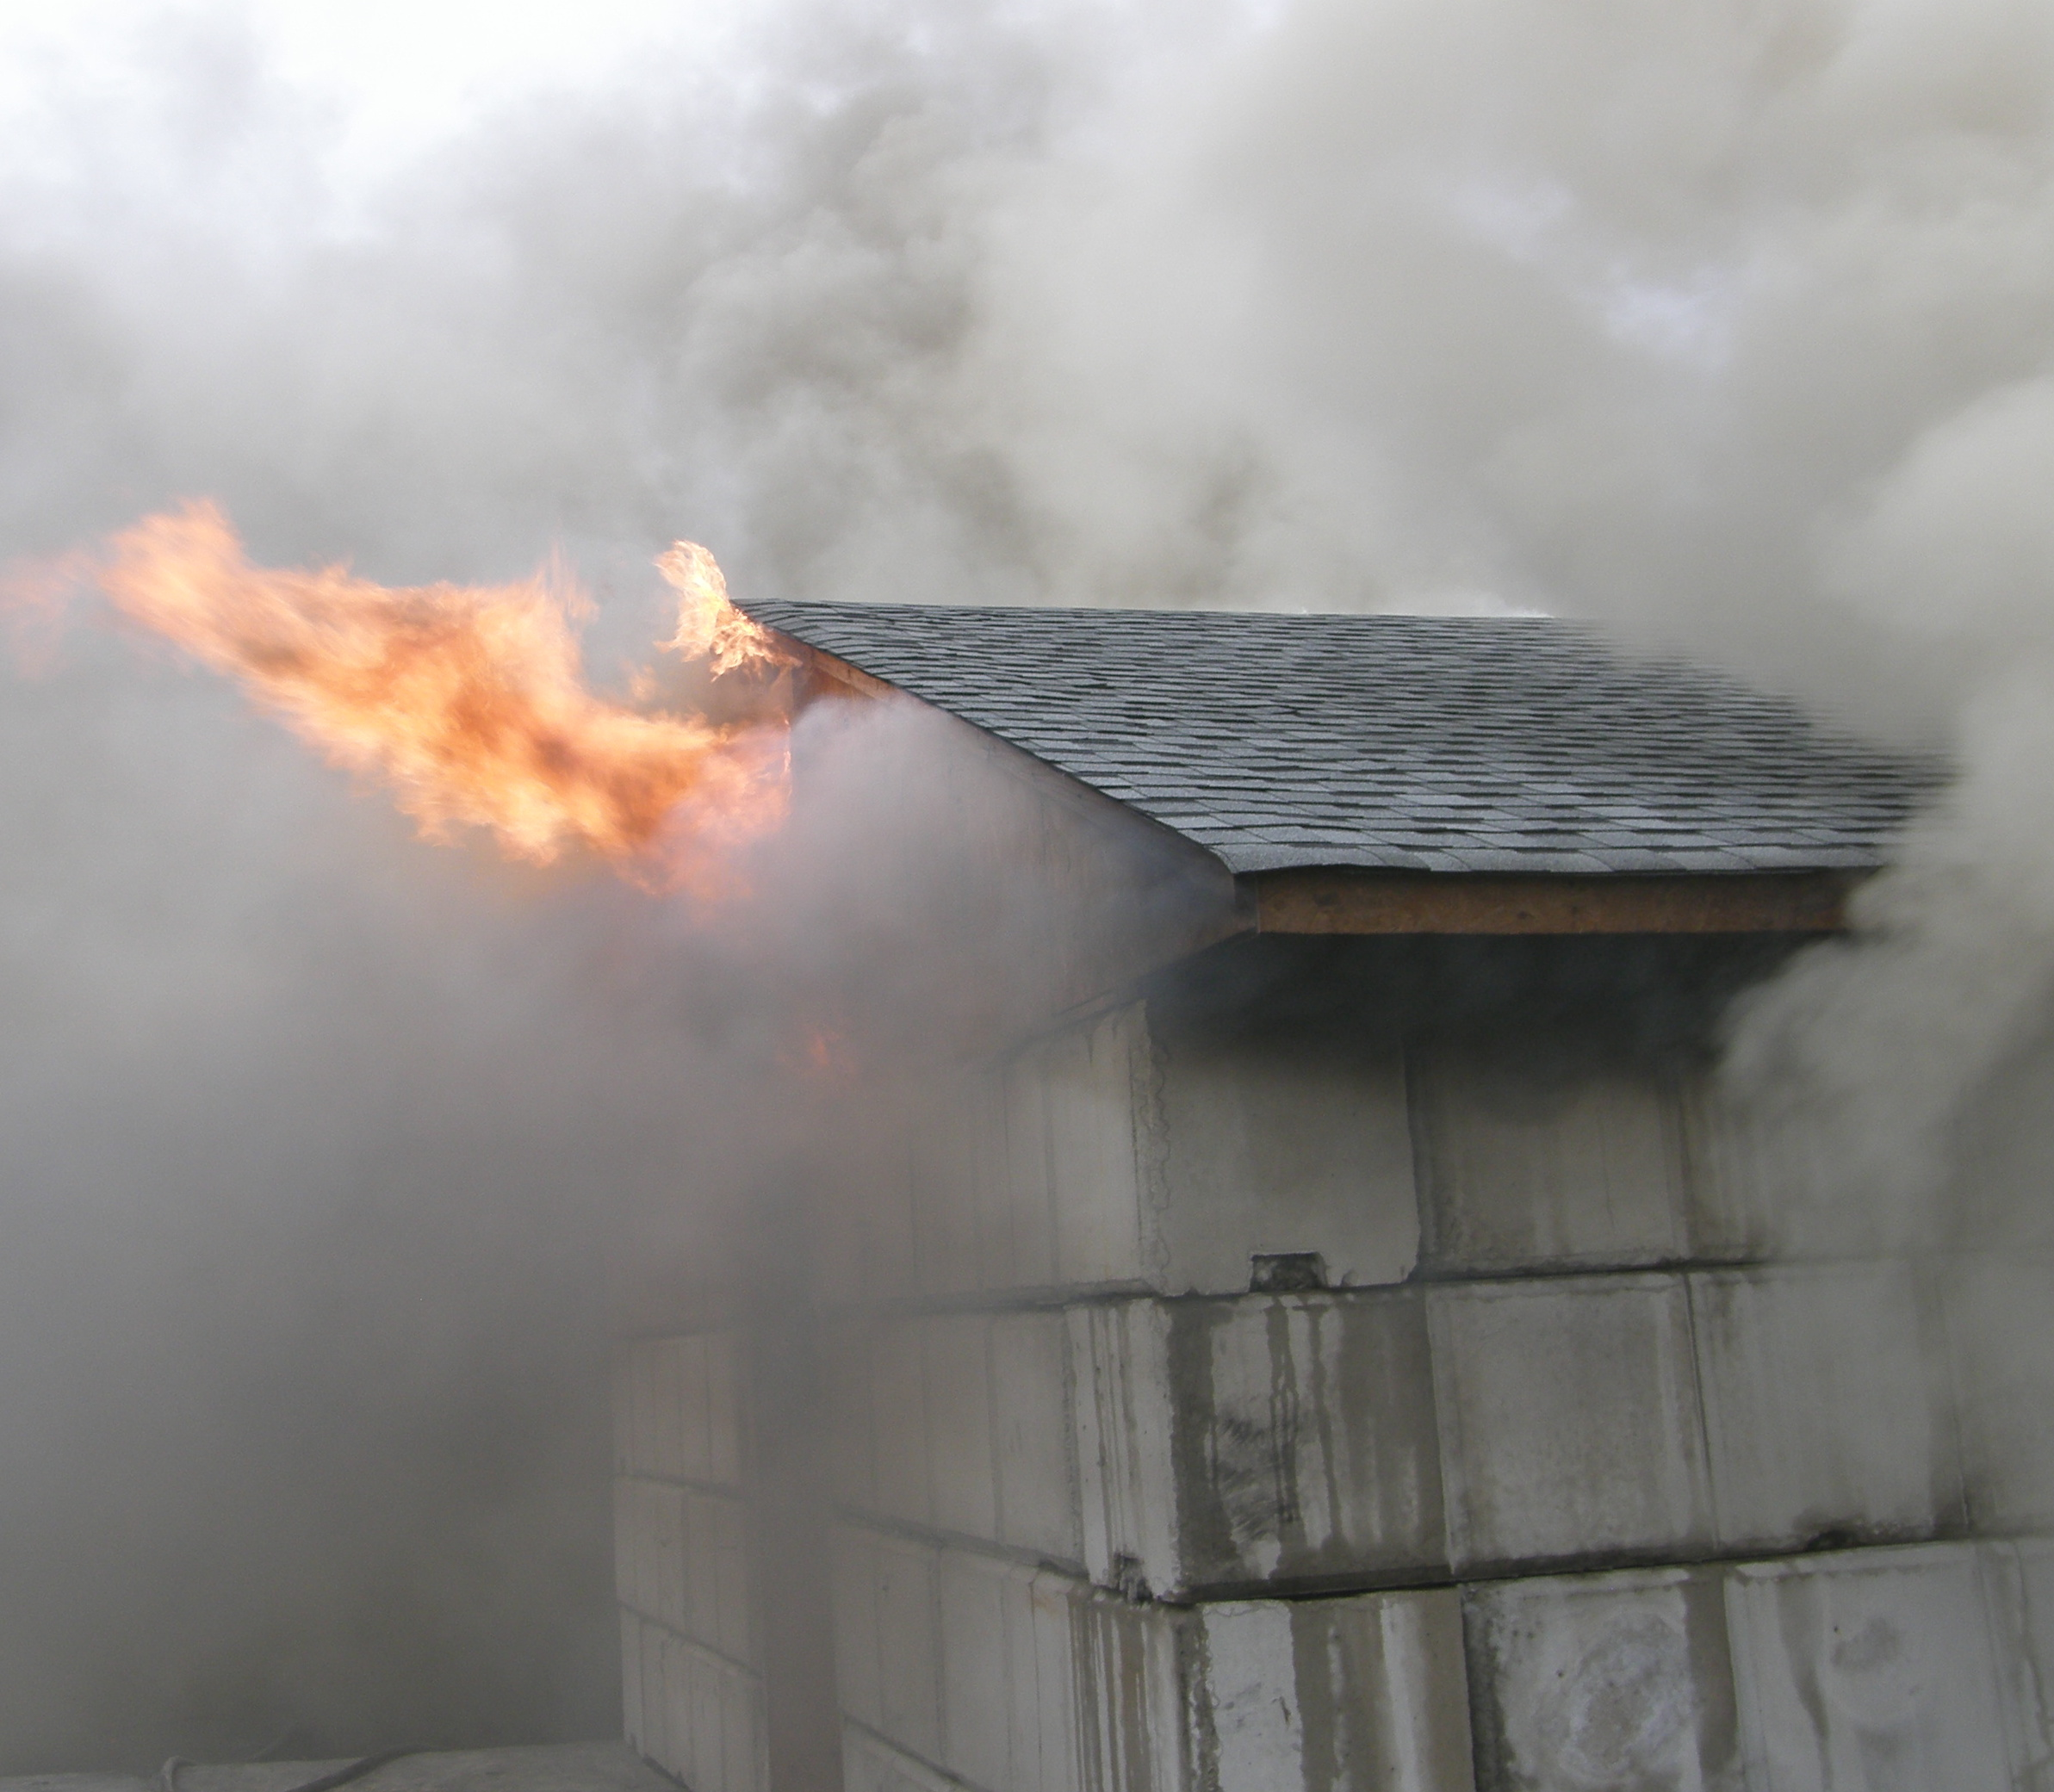
\includegraphics[width=.6\textwidth]{../Figures/PA020340}
\caption{External buirning throught attic eave}
\label{fig:eave}
\end{figure}

\item The authors discard the secondary simulation based on the similarity of the overall HRR, but an alternative ventilation pattern could potentially alter the flow path inside the building. They should explain in more detail why this is not the case in this scenario (or provide images of the flow path and temperature distributions of the secondary simulation). \\
{\it Text was added to state that in both cases the flow path path was the same and the hazard to the firefighters were similar.}
\item I further think that the beginning of section 5.2 is misleading. Surely second-degree burn injuries are only produced by direct contact with objects at 55C. Air at 55C would not burn the skin. It would be useful to relate the temperatures (gas and wall) to heat fluxes, as this would be a more correct approach in terms of human perception and injuries. \\
{\it The section has been updated.}
\end{itemize}

\section{Comments from Reviewer 2}
\begin{itemize}
 \item The authors mention that the fire was under-ventilated yet the species that they have used in the analysis are well ventilated values.  Although the results of the modelling will not be effected by the assumed fuel, the precedent set in this paper could be used by others to justify these as appropriate values for under-ventilated fire when clearly they are not.  Additional discussion on the species and why the well ventilated values used are appropriate for this analysis but should not be used when modelling under-ventilated fire. \\
{\it Good points! Additional discussion was added to the report after the chemical reaction and yeilds were specified.}
\item The authors used 50kW/m2 for calculating there maximum heat release rate yet this value is lower than expected.  The author should explain why this low value was chosen.  The authors then go on and use a HRRPUA=2250kW/m2.  Why did not use the original 50kW/m2 and expand the area burning?  Additional explanation would be helpful. \\
{\it The 50 kW/m2 is a conservative estimate for the HRRPUA. In reality the fire might have been larger - but even a fire of this size produced high hazard conditions for firefighters. There is discussion added to the report. In the attic, there could have been a larger burning area with smaller heat release rate but a compromise was made for Q* and D*.}
\item This results in a floor area of approximately 105 m2 (1100 ft2) per floor and a main living area of approximately 110 m2 (2200 ft2).
The 110m2 should be 210m2??? \\
{\it Thanks for the keen eye. Typo is corrected.}
\item  Around the time of the incident inside the building, E49 attic window.  It is not clear if this was an attic window or the window from the 2nd floor enclosed porch where the fire was.  Urban legend has it that a fire can be pushed through a structure with a hoseline.  Some discussion why this was discounted would be helpful to the reader. \\
{\it The authors recognize that many in the fire service believe fire can be pushed with water but disagree with that legend. A properly applied straight stream or smooth bore stream will not push fire. A wide fog nozzle when applied from the exterior can create a pressure boundary condition at the vent and force hot combustion gas to an area of lower pressure. The text in the tactical consideerations section has been update to include discussion that applying water from the exterior can make conditions better for firefighters.}
\item There was a firefighter with the Captain that perished in the fire.  What were his injuries and location if known?  Some discussion about this 2nd firefighter in the area would be useful. \\
{\it The firefighter with the Captain was not seriously injured.}
\item The condition of the door clearly shows significant damage to the metal door yet the temperatures modelled in FDS are only 260°C.   Is this an artefact of Smokeview's colorbar?  What was the temperature in the porch area when the door is thought to failed?\\
{\it The authors set these bounds because 500~$^{\circ}$F is the upper limit for firefighter PPE. There is discussion of this after the first temperature figure. Text was added to include temperatures on the fire side of the door prior to failure.}
\end{itemize}


\section{Comments from Reviewer 3}
\begin{itemize}
\item It is interesting that the roof is vented at 17:27 right as the Mayday is called.  I suspect that it is a coincidence as there doesn't appear to have been 30-60 seconds for any change in the flow path caused by that action to propagate...but it might be worth inclusion in Table 1 and/or a little discussion. \\
{\it The roof vent was completed when they heard the MayDay. The door failed and the flow path was established before the MayDay was called therefore the roof vent was not a major factor. The last communication from E123 Captain was at 17:23 which is included in Table 1.}
\item Page 6.  With the discussion of the specified fire size, I was left wondering if that would be vent limited by the model.  It turns out it was, and you covered that well...but perhaps a note in this section mentioning that might be nice. \\
{\it At the stage of the discussion, the model results are not yet presented. There has been additional discussion added here based on other comments though.}
\item Page 16 line 40-41.  If there is a reference available for the NIST testing looking at the post-fire state of doors (as shown in Figure 15) it would be nice to provide that here. (or perhaps if unpublished just footnote the person who did the testing so readers know who they could ask for further info) \\
{\it A footnote has been added with a webadress where the report will live upon publication}
\end{itemize}

\section{Comments from Reviewer 4}
\begin{itemize}
\item Are the simulation input files going to be available somewhere online or with the publication? If so, that could resolve a number of these issues and the paper should have a reference to the location of these input files. \\
{\it The main input file will be provided as part of the Fire Technology electronic submission process. Additionally, all the files used to generate the simulations and report will be avilable through an open-source repository. At this current time, google-code is shutting down. The repository has yet to be migrated but I can provide that location upon request once it finds a new home.}
\item  The abstract reference to fire spread to the 2nd floor does not necessarily make it clear that the spread is from the attic in the downward direction. It could be clarified by adding a statement that there was no fire on the first [ground] level. [see p. 1] \\
{\it The abstract was clarified to indicate the fire spread downward and that there was no fire damage on the first floor.}
\item At the end of introduction to section 3, it would be good to put a reference to the SFPE Guide to Selecting a Fire Model for a Particular Purpose and that the authors considered the relevant physics and output to decide to use FDS. [See p. 4] \\
{\it Discussion was added referring to the SFPE Guide}
\item  Section 3.3 Materials would be more helpful if it also more fully addressed the exterior walls. I am expecting these were modeled just with gypsum board given the descriptions, rather than some sort of sandwich or other heat transfer approach. [See p. 7] \\
{\it Added discussion.}
\item Section 3.3 Materials should also address what was done with the windows. No description of glass was given, so this should be addressed explicitly. [See p. 7] \\
{\it That is correct. This is clarified in the text.}
\item The vents are unclear to me [See Tab. 2 and accompanying text, p. 7]. For example, which vents are the ones that were cut into the roof to vent the attic? In addition, I don't see any vents in the figure of the roof [See, for example, Fig. 5, p. 9]. \\
{\it You are correct in that there were roof ventilation holes that were made. Roof ventilation occured after the interior flow path was established and was not considered in the model.}
\item Vents: Were all of the windows considered closed? I did not find that directly stated, especially given the details about all of the windows in the last two diagrams. \\
{\it Addressed related to prior comment.}
\item Vents: Where is the connection between the 2nd floor porch and attic? I saw it described broadly in the paper, but don't recall it being described more fully and it is not depicted in any of the diagrams. \\
{\it Addtional text was added describing the stair connecting the porch to the attic.}
\item Vents: Table 2, p. 7, it would be helpful to have a quick description of what each vent is in terms of the fire incident report. \\
{\it These vents were found by watching a video of the incident. Besides the door opening they do not tie into the narrative from NIOSH.}
\item On the numerical resolution examination [see p. 8, lines 22-27], it would be helpful to explain that higher numbers equate to better resolution as the non-user may not appreciate this and think that being outside the range makes it an unreliable calculation. \\
{\it Text added to clarify.}
\item HRR: The graphic [Fig. 6, p.10] is fine and accompanying text is also good. One thing that is not clear, but may be helpful to the reader is to explain that some of that combustion is occurring outside the structure [See Fig. 7, p. 12]. This is important given the discussion of temperatures, etc. If the authors know the amount of HRR within the structure, that may be an interesting/helpful value for the readers. \\
{\it Addressed by other reviewer's comments. See section in text.}
\item Attic fire: Was any of the roof ``consumed?'' [See Fig. 7, p. 12 and associated text] It would be interesting to know if any of the roof was ultimately consumed and whether that occurred subsequent to the modeled period or if there was another reason to disregard that phenomenon. [See Fig. 2, p. 6]\\
{\it The authors used video evidence to examine the breaches through the structure from the fire prior to the MayDay call. At that time there was no breach through the roof. Post incident there were holes cut by the fire service as well as some that might have been caused by the fire but we do not have enough evidence to make a difinitive assessment.}
\item Pressure: Section 4.2 [See p. 12, line 30] discusses over-pressure. I am unclear about that particular part of the discussion. The text references``at 1 m'', but I think this could be more clear that you are not talking about a compartment over-pressure, but that generated by buoyancy due to temperature differences. I don't think the authors mean that the whole compartment is over-pressured. This is an important distinction, because later the discussion focuses on the door, but I am under the impression that the door folding is heat caused structural failure, not overpressure. Therefore, it's important to clarify this point.
{\it Excellent point. This is clarified.}
\item Pressure: [See Fig. 8, p. 12] I am unsure how to interpret this graphic as presumably there are some lower pressures driving air into the various spaces as normal gravity flows. I think this figure should have some additional description to better explain what it's showing. Somewhere, there must be air entering these various spaces in order to continue combustion in those volumes. \\
{\it Discussion added to Pressure section.}
\item Fig. 14, p. 16: This photo shows the door and discusses the crease, which I can see. I assume from my reading that this is the interior face of the door and that the top of the door is towards the background. This should be clarified in the caption. \\
{\it Clarified in the text.}
\item Fig. 20, p. 24 \& Fig. 21, p. 25: These graphics are good overall. Unfortunately, the cross-hatching is difficult to interpret in some places. Furthermore, it will be impossible to read this if it is reproduced in black and white. \\
{\it Images were removed to address excess figures but a reference was made to report where figures live.}
\item  It would be helpful to have a floor plan of the attic space that includes the locations of the roof vents. \\
{\it Because of post-incident safety concerns we were unable to measure the attic or get accurate location of roof vents. Note that these vents were made after the interior door failed.}
\end{itemize}

\end{document}
